Most of our experiments are based on the simulation described in section
\ref{sec:simulation} as our code is not performant enough to handle the amount
of events a real dynamic vision sensor generates and because the simulation
makes comparisons with ground truth much easier.

There are a few things we looked into with the real DVS tough:

\subsection{initialization by removing shutter}

If the DVS is fully covered by a shutter we can recover a full picture by
simply removing it slowly and integrating all the events generated. This allows
for an easy initialization of the map using only the DVS. An example is shown in Figure \ref{fig:shutter_integration}

\begin{figure}
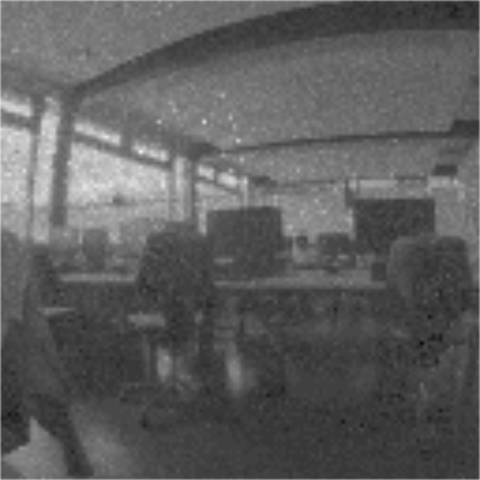
\includegraphics[width=\linewidth]{images/PCLab_integrated.png}
\caption{image of our lab generated by integrating over short interval while removing shutter}
\label{fig:shutter_integration}
\end{figure}


\subsection{camera calibration}

As with any sensor, we must calibrate the DVS to get usable data. For normal
cameras, this is usally done by capturing images of a checkerboard pattern from
different viewpoints and subsequently rectifying images so they fit into a
standard pinhole camera model.

Unfortunately, the dynamic vision sensor only detects changes and cannot
directly capture a calibration pattern. We could take pictures as described in
the previous section, but for calibration there is an even better method \cite{mueggler2014event}: Use a
computer screen to quickly show and hide the pattern. This is not only quicker
and more convenient than removing a shutter, it also has the advantage of only
showing the pattern and none of the surrounding scenery.

This method can also be used to focus the camera optics by displaying a pattern
of lines with varying sizes.

\begin{figure}
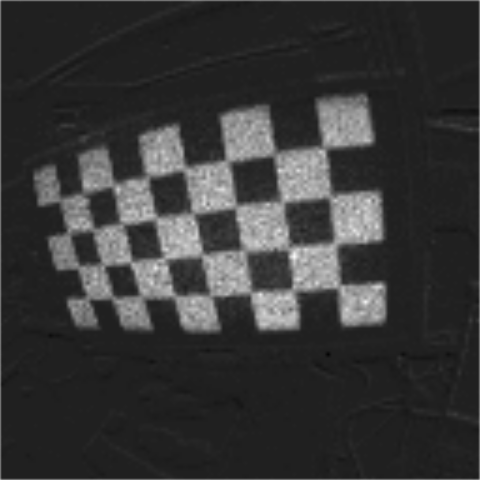
\includegraphics[width=\linewidth]{images/checkerboard_integrated.png}
\caption{a sample checkerboard pattern used for calibration}
\label{fig:calibration}
\end{figure}
